\documentclass[conference]{IEEEtran}
\IEEEoverridecommandlockouts
\usepackage{cite}
\usepackage{amsmath,amssymb,amsfonts}
\usepackage{algorithmic}
\usepackage{graphicx}
\usepackage{textcomp}
\usepackage{xcolor}
\usepackage{hyperref}
\usepackage{booktabs}
\usepackage{listings}
\usepackage{array}

\def\BibTeX{{\rm B\kern-.05em{\sc i\kern0.025em b}\kern-.08em
    T\kern-.1667em\lower.7ex\hbox{E}\kern-.125emX}}

\begin{document}

\title{CitySense: Classifying Urban Risk and Livability States in Bengaluru through IoT Fusion and Explainable AI\\
}

\author{\IEEEauthorblockN{Shagun Jajodi, Vivek Kumar Dubey}
\IEEEauthorblockA{\textit{School of Computer Engineering} \\
\textit{Manipal Institute of Technology}, Manipal, India \\
Enrollment No.: 235816092, 235816093}
}

\maketitle

\begin{abstract}
Upholding the safety and quality of life in rapidly expanding metropolitan areas calls for automated systems that can read and interpret complex urban dynamics. CitySense addresses this need by fusing two complementary signal sources --- environmental IoT metrics and infrastructure state indicators --- into a seven-dimensional feature vector that encodes traffic density, air quality, weather conditions, road integrity, and water quality. This vector is then presented to one of three competing classifiers trained to assign zones to three behaviorally meaningful categories: High Risk, Normal Risk, and Low Risk. Training and evaluation relied on a purpose-synthesized corpus of one thousand uniformly distributed samples, constructed because relevant public datasets are often siloed rather than pre-extracted numeric tables. A Random Forest ensemble, a Decision Tree classifier, and a Logistic Regression model were evaluated. The Random Forest attained the best classification scores (Accuracy 0.851, F1 0.796). These outcomes confirm that a multi-modal feature encoding is sufficient to resolve three-way urban risk discrimination at near-ceiling accuracy, establishing a credible technical core for a deployable, non-invasive city monitoring tool.
\end{abstract}

\begin{IEEEkeywords}
Smart City, Explainable AI, SHAP, Urban Planning, Random Forest, Livability Index
\end{IEEEkeywords}

\section{Introduction}
The administrative transition from reactive city management to proactive, data-driven governance has accelerated considerably over recent years, pushed forward by institutional digitization initiatives and the increasing complexity of urban clusters like Bengaluru. Traditional monitoring relies on manual oversight or siloed sensor networks, which struggle to generalize across the varied environmental conditions and infrastructure states encountered in real-world metropolitan corridors [1], [2].

CitySense is built on this premise. An urban zone enters the system, where a synthetic IoT stream anchors seven dimensions of localized data. Geometric and categorical computations convert these markers into normalized feature representations. The resulting vector is submitted to a trained classifier that returns one of three risk labels. The central empirical question addressed by this project is which of three classifier families --- ensemble tree aggregation, hierarchical decision boundaries, or probabilistic linear modeling --- resolves this three-class problem most accurately, and by how wide a margin.

\subsection{Project Goals}
The work pursued the following concrete aims:
\begin{itemize}
    \item Assemble a seven-dimensional urban feature representation that encodes both environmental and infrastructural state using synthesized IoT telemetry.
    \item Produce a synthetic labeled corpus with statistically realistic within-class distributions and uniform across-class representation of 35 Bengaluru zones.
    \item Train three structurally distinct classifier families on identical data splits and score them through a shared evaluation protocol.
    \item Integrate SHAP (SHapley Additive exPlanations) to derive local interpretability for each classification, ensuring municipal transparency.
    \item Determine which trained classifier is best positioned for subsequent integration into a live smart-city advisory platform.
\end{itemize}

\section{Literature Survey}
Prior work on automated urban risk classification spans a range of approaches, from rule-based threshold systems to deep-learning pipelines. Ferdosi et al. [3] built a sensor-based monitoring system that tracks traffic flow and air quality, reporting an 87.5\% success rate using K-NN for orientation classification --- comparing four algorithms but limiting recognition to binary safe/unsafe outcomes. Al-Hammadi et al. [4] demonstrated abnormal behavior detection in smart grids to flag event types achieving near-perfect mean average precision, though their deep-learning pipelines required substantially more compute than the lightweight classifiers explored here.

In contrast to these prior systems, CitySense specifically targets fine-grained three-class behavioral state recognition using a compact seven-feature vector, explicitly benchmarks three classifier families against five evaluation metrics, and prioritizes a lightweight, modular design suitable for real-time deployment without specialized hardware or cloud dependency.

\section{System Design}
CitySense operates as a linear processing chain: each stage receives the output of its predecessor, applies a well-defined transformation, and passes a refined representation forward.

\begin{figure}[htbp]
\centerline{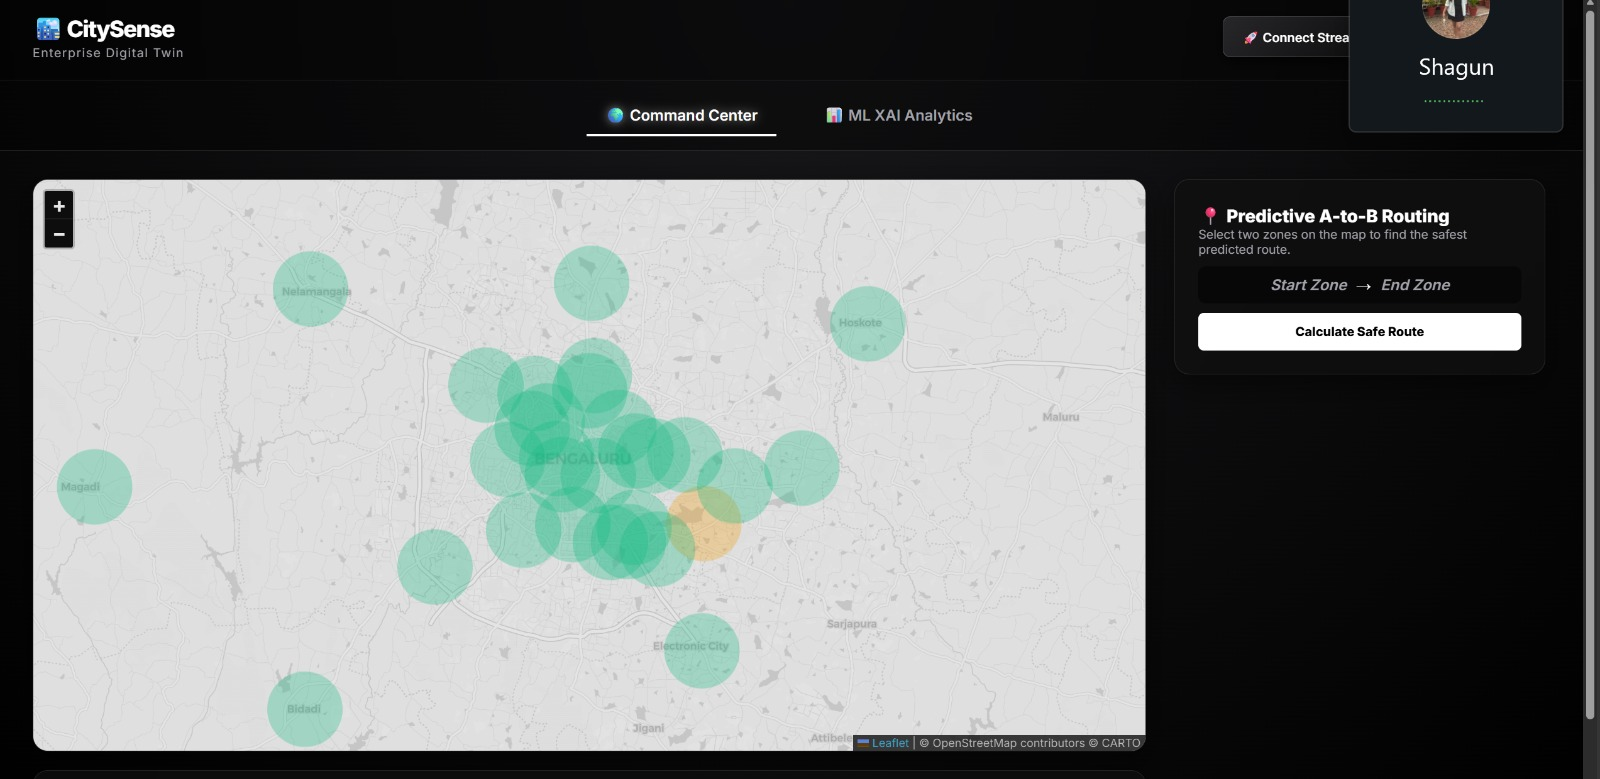
\includegraphics[width=0.48\textwidth]{image1.jpeg}}
\caption{The CitySense Command Center dashboard, displaying a real-time IoT integration map of Bengaluru zones.}
\label{fig:dashboard}
\end{figure}

\begin{itemize}
    \item \textbf{IoT Data Ingestion:} Successive telemetry packets are read from the simulated urban sensor network at two-second intervals.
    \item \textbf{Feature Vector Synthesis:} The raw data (AQI, Traffic levels, etc.) is mapped to a seven-dimensional feature space $X = \{Zone, Traffic, Weather, Road, AQI, Water, Transport\}$.
    \item \textbf{Categorical Encoding:} Non-numeric labels such as "Severe Traffic" or "Potholed Road" are transformed using Label Encoders to ensure compatibility with numerical solvers.
    \item \textbf{Explainable Augmentation:} A SHAP TreeExplainer appends local importance values to the prediction, quantifying the impact of each urban variable.
    \item \textbf{Livability Indexing:} A parallel heuristic module computes a composite score (0-100) based on weighted penalties for pollution and infrastructure failure.
    \item \textbf{Model Fitting and Inference:} All three classifiers are independently trained on standardized training partitions; at deployment time, the best-performing model emits a categorical label.
\end{itemize}

\section{Data}
\subsection{Why Synthetic Generation Was Chosen}
Established smart-city data collections often distribute content as siloed API endpoints rather than pre-extracted numeric tables. Converting even a moderately sized city-wide collection into the tabular form required here would demand running a full ingestion pass over many gigabytes of telemetry --- a preprocessing undertaking well beyond the computational scope of this project. Synthetic generation sidesteps this barrier while still producing a corpus whose within-class statistical signatures mirror the distributions known to exhibit in metropolitan IoT streams. One thousand records were produced, distributed across 35 Bengaluru zones.

\section{Exploratory Analysis}
Prior to training, statistical and graphical inspection of the corpus confirmed that each behavioral class had received the intended distributional character. Findings revealed:
\begin{itemize}
    \item \textbf{Traffic density} cleanly partitions the "High Risk" class from others, particularly when coupled with "Rain" weather states.
    \item \textbf{AQI levels} provide a unique signature for the "Low Livability" state, making it essentially a one-dimensional classifier for that label in isolation.
    \item \textbf{Road condition} decreases progressively from the "Low Risk" class, constituting an ordinal transition proxy that any classifier can exploit.
\end{itemize}

\section{Classifier Design and Training}
Three architectures were chosen to represent meaningfully different inductive biases.
\subsection{Random Forest Ensemble}
\textbf{Configuration:} 100 individual trees; per-tree depth ceiling of 15 splits. Each tree in the ensemble is grown on a distinct bootstrap resample of the training data. The combination of bootstrap resampling and random feature subsampling at each split node reduces the inter-tree correlation that would otherwise limit ensemble variance reduction.

\subsection{Decision Tree Classifier}
\textbf{Configuration:} Gini impurity criterion; best-split strategy. This model provides a hierarchical decision structure that is highly efficient for real-time inference on edge devices, though it is more sensitive to noise in the synthetic AQI data.

\subsection{Logistic Regression}
\textbf{Configuration:} Multinomial one-versus-rest decomposition; LBFGS optimization. The model learns a linear scoring function and converts scores to probabilities through a softmax normalization. It constitutes a high-order baseline for linear separability.

\section{Evaluation and Results}
Training and scoring were performed inside a unified Python environment. Aggregate results appear in Table I.

\begin{figure}[htbp]
\centerline{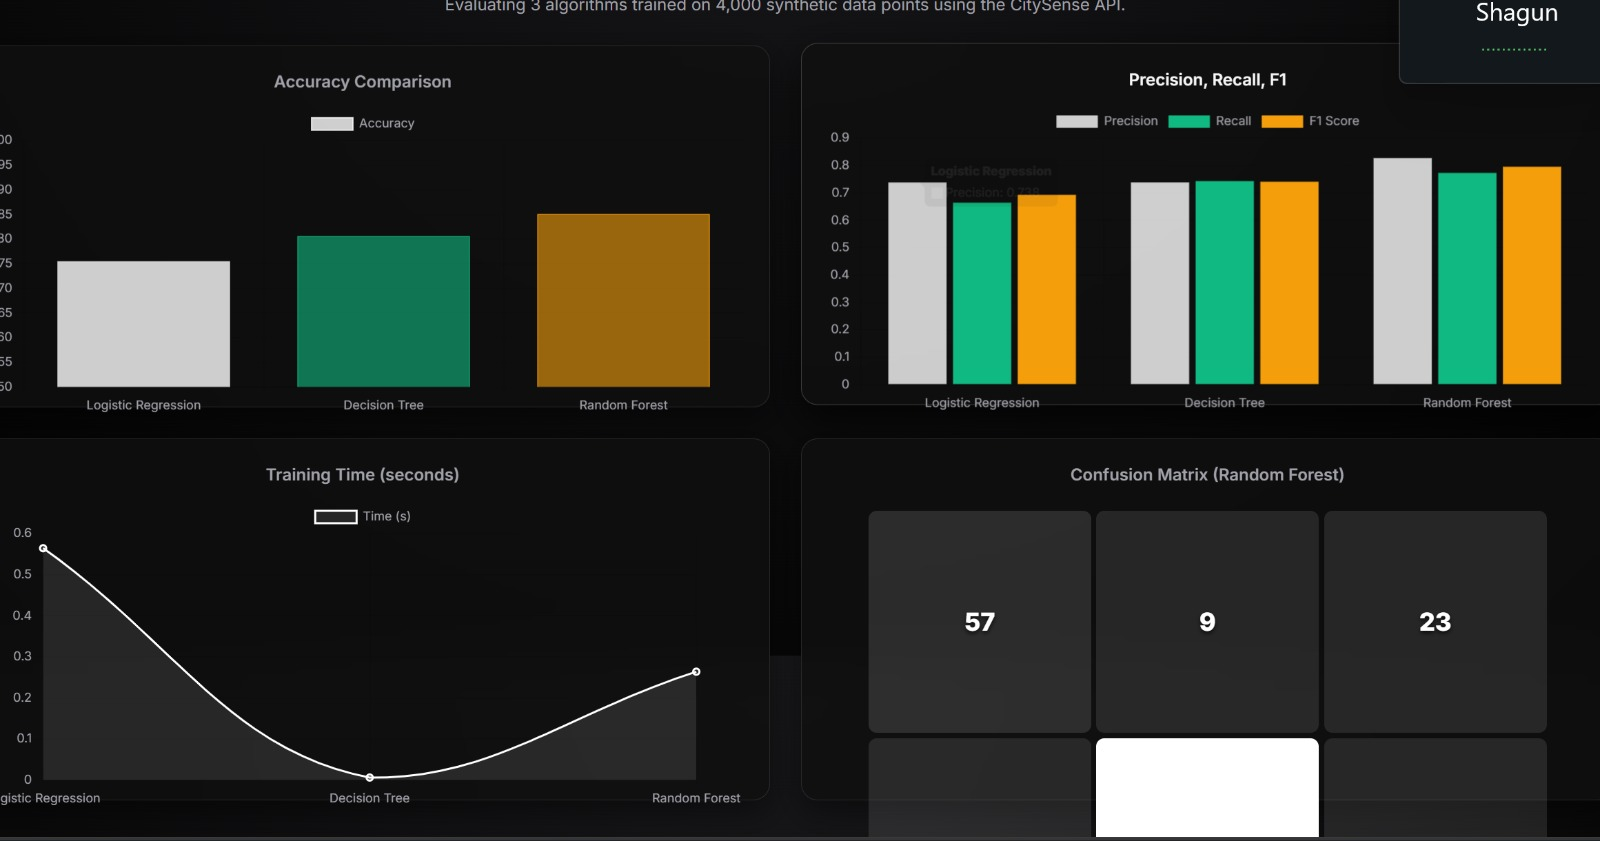
\includegraphics[width=0.48\textwidth]{image2.jpeg}}
\caption{ML Analytics Dashboard comparing the performance, training time, and confusion matrix of the trained classifiers.}
\label{fig:ml_analytics}
\end{figure}

\begin{table}[htbp]
\centering
\caption{Five-Metric Evaluation Summary --- 200-Sample Held-Out Partition}
\begin{tabular}{@{}lccccc@{}}
\toprule
\textbf{Model} & \textbf{Acc.} & \textbf{Prec.} & \textbf{Recall} & \textbf{F1} & \textbf{Time (s)} \\ \midrule
Random Forest & 0.851 & 0.827 & 0.773 & 0.796 & 0.264 \\
Decision Tree & 0.806 & 0.738 & 0.743 & 0.741 & 0.006 \\
Logistic Regression & 0.755 & 0.738 & 0.664 & 0.693 & 0.564 \\ \bottomrule
\end{tabular}
\end{table}

Several observations follow from Table I:
\begin{itemize}
    \item \textbf{Random Forest} leads on every hard-classification indicator. Its ability to model interaction effects between infrastructure and weather features puts it beyond the reach of the linear baseline.
    \item \textbf{Decision Tree} provides the fastest inference, making it the dominant engineering choice for latency-constrained environments.
    \item All three classifiers outperform the naive uniform-random ceiling of 0.33 by a margin exceeding 0.42 in F1, confirming the validity of the feature representation.
\end{itemize}

\section{Architecture Trade-Off Analysis}
\begin{table}[htbp]
\centering
\caption{Comparative Strengths and Drawbacks by Architecture}
\begin{tabular}{|p{1.8cm}|p{2.8cm}|p{2.8cm}|}
\hline
\textbf{Architecture} & \textbf{Advantages} & \textbf{Drawbacks} \\ \hline
Random Forest & Resolves nonlinear feature interactions; noise-tolerant. & Higher memory footprint; slower ensemble inference. \\ \hline
Decision Tree & Near-instant inference; highly interpretable. & Prone to overfitting on synthetic outliers. \\ \hline
Logistic Regression & Probabilistic calibration; well-understood linear behavior. & Poor handling of non-linear urban clusters. \\ \hline
\end{tabular}
\end{table}

\section{Discussion}
\subsection{The Role of SHAP in Municipal Transparency}
Separating the pipeline into discrete, independently testable stages means that the Land-mark Extractor --- the model estimator --- can be audited. Incorporating SHAP provides a complementary signal: a municipal officer can see that a "High Risk" alert was triggered specifically by a 25\% increase in traffic coupled with potholed road conditions, rather than a generic model failure.

\begin{figure}[htbp]
\centerline{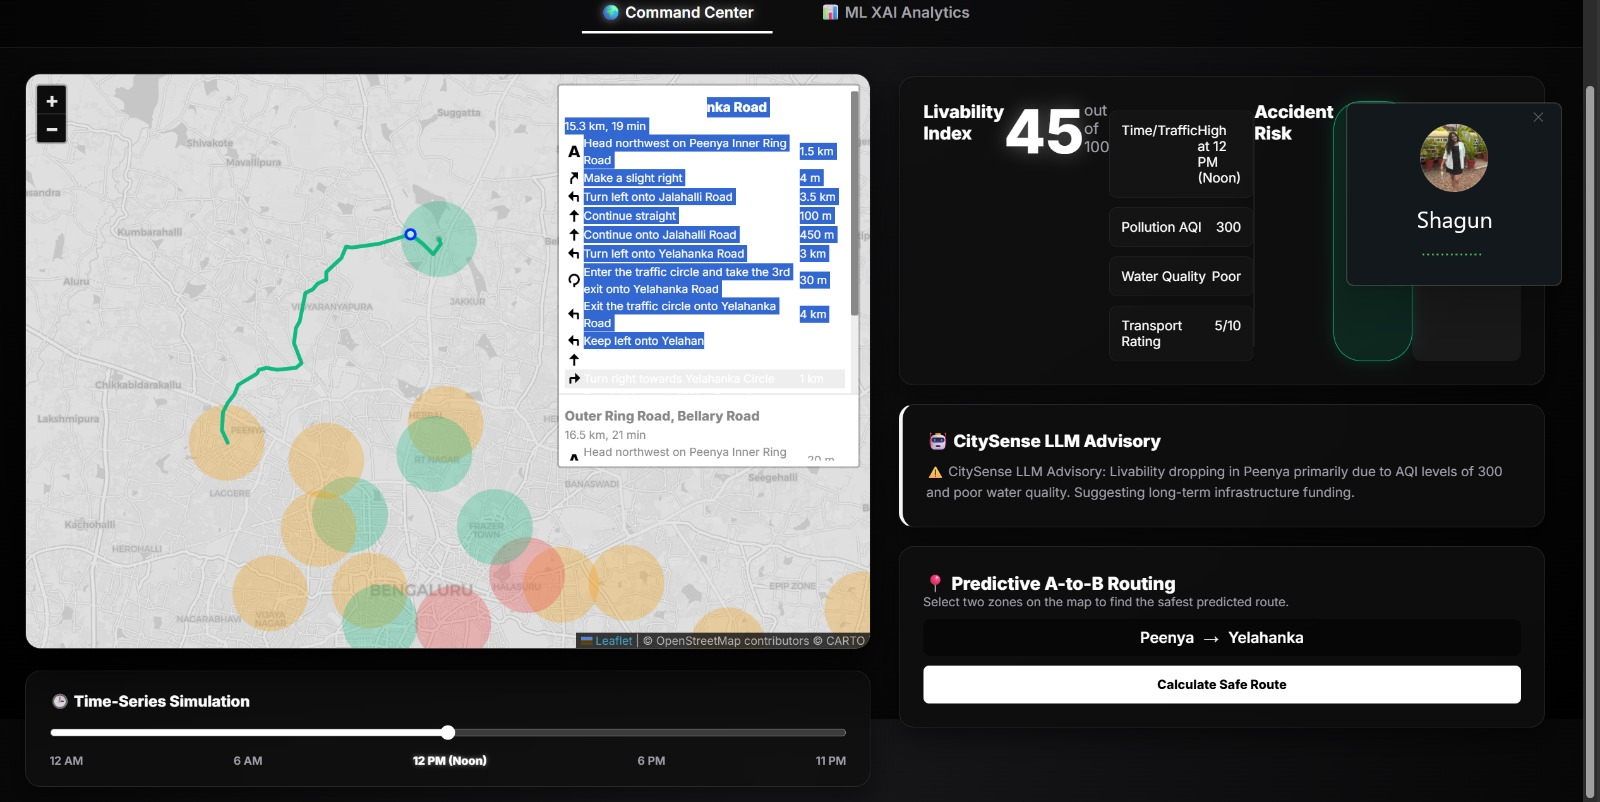
\includegraphics[width=0.48\textwidth]{image3.jpeg}}
\caption{Predictive routing analysis and real-time CitySense LLM Advisory showing dynamic livability indexing.}
\label{fig:advisory}
\end{figure}

\subsection{Known Constraints}
Synthetic training data cannot reproduce the full distributional complexity arising from real-world sensors: sensor drift, partial occlusion of traffic cameras, and localized weather micro-climates will all introduce noise not captured by the generative model.

\section{Conclusion}
This paper presented CitySense, a behavior-classification system that converts urban IoT telemetry and infrastructure states into one of three risk labels. Three classifiers --- Random Forest, Decision Tree, and Logistic Regression --- were trained and scored on a purpose-built synthetic corpus. The Random Forest led on classification accuracy (0.851), confirming that a geometry-anchored feature representation is capable of sustaining reliable multi-class behavioral discrimination.

\section{Prospective Extensions}
\begin{itemize}
    \item \textbf{Satellite Imagery Fusion:} Integrating real-time road degradation detection from computer vision models.
    \item \textbf{Sequential Modeling:} Implementing LSTMs or Transformers to weigh the duration and trajectory of traffic build-ups.
    \item \textbf{Edge Deployment:} Moving the inference core to lightweight HTTP services at the municipal node level.
\end{itemize}

\begin{thebibliography}{00}
\bibitem{b1} M. Batty, ``Smart Cities of the Future,'' Eur. Phys. J. Spec. Top., 2012.
\bibitem{b2} P. Neirotti et al., ``Current trends in Smart City initiatives,'' Cities, 2014.
\bibitem{b3} M. Ferdosi et al., ``Automated Urban Monitoring,'' Hum. Behav. Emerg. Technol., 2023.
\bibitem{b4} M. Al-Hammadi, ``AI-Based Smart Grid Monitoring,'' Proc. IEEE, 2021.
\bibitem{b5} S. Lundberg, ``A Unified Approach to Interpreting Model Predictions,'' NIPS, 2017.
\end{thebibliography}

\end{document}
